\chapter{Introducción}

En una era digital donde las tendencias cambian en un abrir y cerrar de ojos, los memes se han convertido en una forma popular de comunicación que se mantiene atemporal y relevante cambiando y adaptándose por cada tendencia.

Los memes están tan integrados en nuestra cultura que los utiliza desde el estudiante que busca hacer sus presentaciones y exposiciones más memorables y llevaderas hasta una empresa que busca captar la atención de audiencia en las redes sociales.

La integración de los memes en el contenido no solo buscan vender el contenido de manera más fresca, entretenida y atractiva, sino que otras veces, solo se busca el entretenimiento y la diversión pura y simple de los consumidores.

Imagine una escena en la que un grupo de amigos se reúne y discuten sobre los últimos acontecimientos políticos cuando, de repente, un meme ingenioso y fuera de lugar se convierte en el centro de la conversación, rompiendo el hielo y generando risas. Imagine ahora una situación, en un entorno académico, en el que un estudiante quiere realizar una presentación algo diferente y para ello decide introducir algún meme. Esta situación no únicamente se da en un entorno académico, sino que incluso en charlas llevadas por ponentes profesionales. Cada vez es más común encontrar algún meme que otro con el fin de que estas charlas sean más `digeribles`. Un claro ejemplo de este caso es Miguel Ángel Durán (\href{https://midu.dev/}{@midudev}), un experto en desarrollo de software, actualmente divulgador sobre programación, estrella de GitHub y Microsoft MVP, el cual es conocido por su habilidad para integrar memes de forma creativa y efectiva en sus charlas y presentaciones.

\begin{figure}[ht]
    \caption{Fotograma sacado del (\href{http://sl.ugr.es/0dXQ}{vídeo de YouTube de la conferencia}): Pierde el miedo a desplegar a producción en viernes | ft @midudev (c) Platzi para la Platzi Conf 2024 en el que se puede ver a Miguel Ángel Durán (\href{https://midu.dev/}{@midudev}) en plena conferencia.}
    \centering
    \vspace*{0.5cm}
    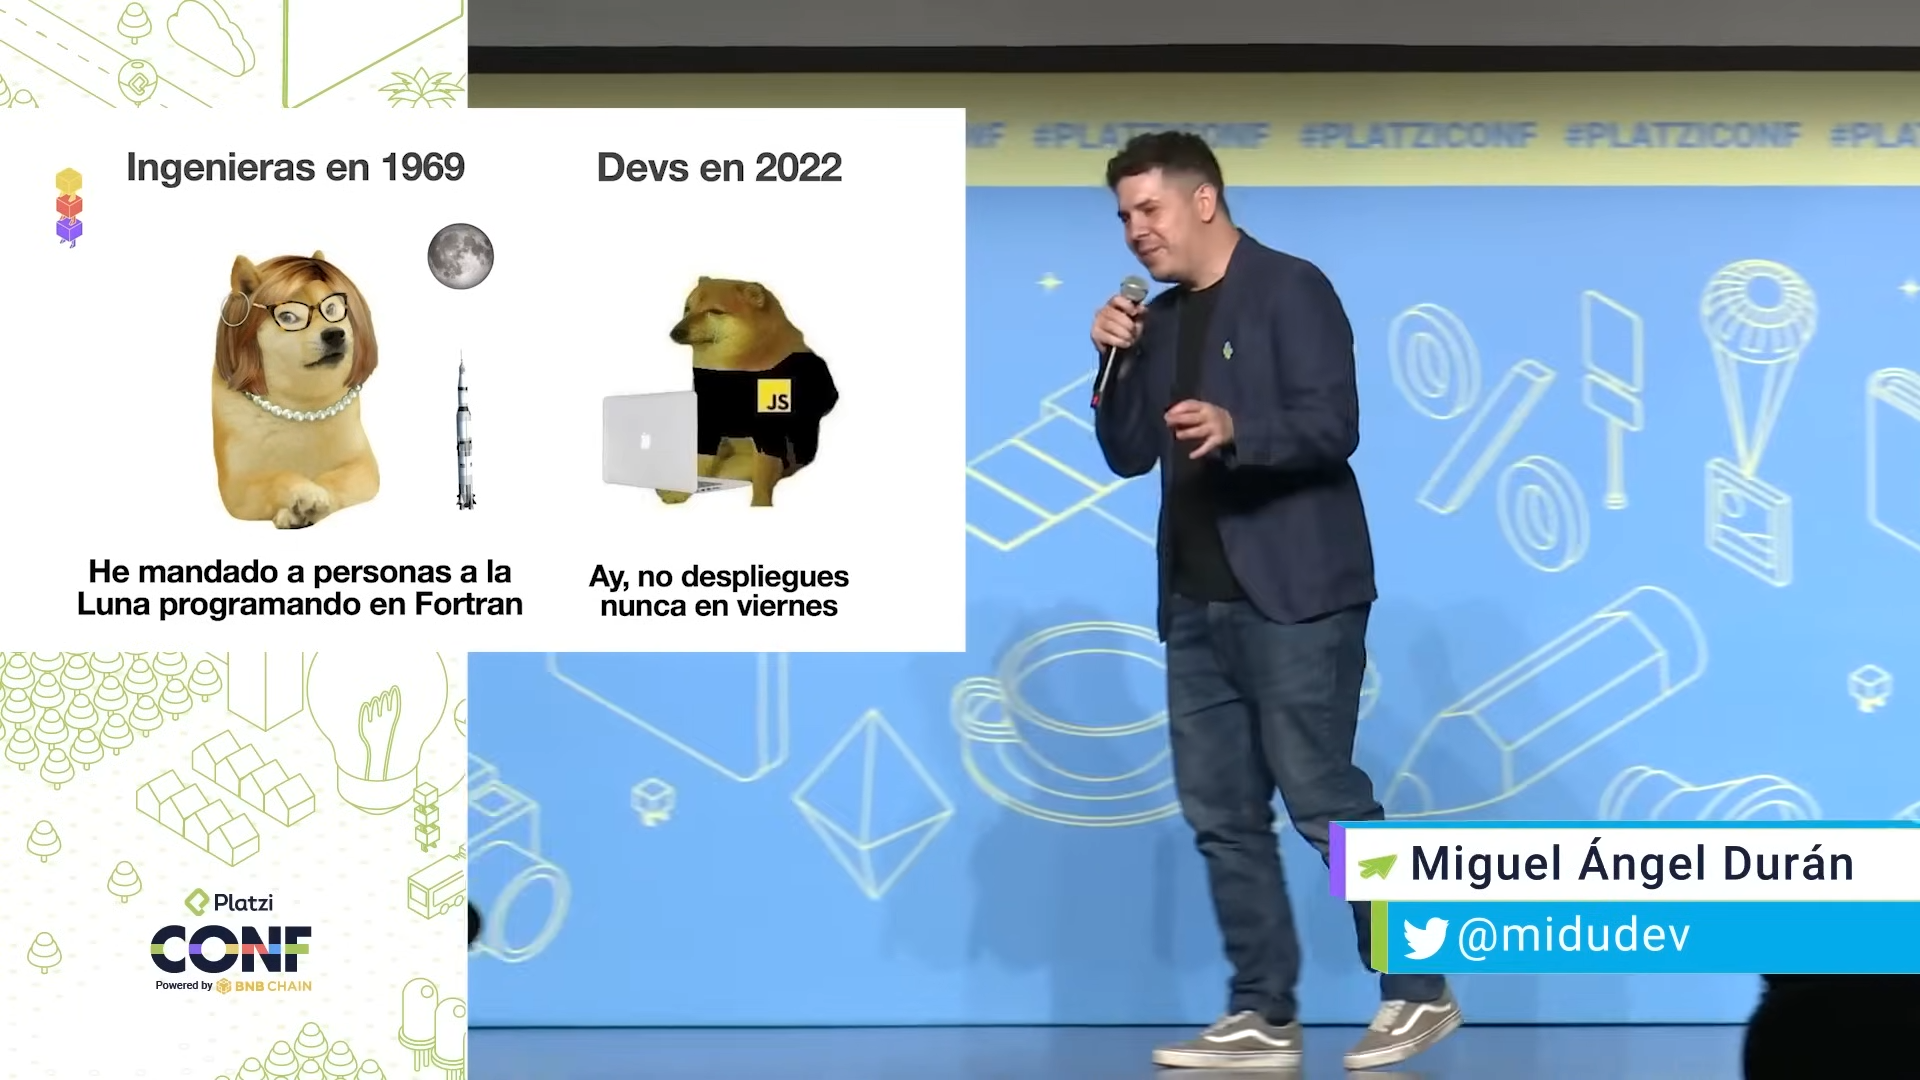
\includegraphics[scale=0.15]{figuras/platziconfmidudev.png}
\end{figure}

En todos estos casos y en muchos más, los memes se han convertido un medio para conectar con el consumidor de una manera única y efectiva.

Sin embargo, a pesar de su uso generalizado, la gestión, centralización y organización de memes sigue siendo un desafío para muchos creadores de contenido, empresas y personas.

\section{Motivación}

Como hemos comentado la creación y compartición de memes es una actividad de lo más habitual por lo que la falta de un sistema centralizado limita su potencial para todo tipo de usuarios. Esta falta de una solución informática específica se traduce en una pérdida de tiempo y recursos, así como en una limitación en la capacidad de generar contenido relevante y oportuno. Lo cual es una característica esencial en el mundo de los memes.

La motivación detrás de este proyecto radica en ofrecer una solución que subsane las dificultades que los usuarios encuentran a la hora de gestionar estos medios de información. Estas dificultades van desde la dificultad de encontrar memes antiguos hasta la falta de herramientas colaborativas y centralizadas. Como se puede apreciar los problemas pueden llegar a ser muy diversos y afectar a diferentes tipos de usuarios.

El proyecto `Memes para todos` aspira a proporcionar una plataforma robusta y fácil de usar que simplifique el proceso de creación, almacenamiento y distribución de memes para todo tipo de usuarios, sin importar su experiencia previa o contexto.

\section{Definición del problema}

Dentro de este marco de trabajo, para realizar una mejor de definición del problema, se han identificado una serie de personas con necesidades y objetivos específicos que junto con las historias de usuario describen los problemas que se pretenden resolver con este proyecto.

La metodología utilizada ha sido la de `personas`. Esta técnica se basa en la representación ficticia, pero concreta del grupo de usuarios al que va dirigido nuestra solución. El fin de este análisis es el poder llevar a cabo una compresión clara de los objetivos y necesidades de los usuarios en contextos específicos de uso \cite{cooper2014face}.

\subsection{Usuarios identificados}

    La identificación de los usuarios es un paso fundamental para el desarrollo del proyecto, ya que permite definir mejor las necesidades, requisitos, deseos, expectativas del usuario final que hará empleo de la solución. Además, estos usuarios sirven para la validación de la solución propuesta.

    \subsubsection{Cristina Contreras Márquez (estudiante de ingeniería informática)}

    Cristina Contreras Márquez es una estudiante de ingeniería informática que, como cualquier otro estudiante, necesita hacer presentaciones para exponer sus trabajos. Cristina es una persona creativa que siempre le gusta aportar su esencia a las presentaciones las cuales vuelve únicas y diferentes. Cristina siempre está buscando encontrar una forma fácil y rápida de hacer esos memes que se le van ocurriendo mientras elabora la presentación.

    \subsubsection{Ted Johnson González (experto conferenciante)}

    Ted Johnson González es un experto en oratoria que realiza muchas ponencias y charlas. Ted es un ponente profesional que siempre busca la manera de hacer sus charlas más amenas y entretenidas. La característica diferenciadora e innovadora de sus conferencias es la inclusión de memes que ayudan a reforzar su discurso y aumentar la retención del contenido por parte de la audiencia gracias a la conexión con el meme.

    \subsubsection{Departamento de marketing de Corporate Solutions}

    El departamento de marketing de `Corporate Solutions` le ha expresado al CTO en la empresa, la necesidad de un sistema centralizado para agilizar el proceso de generación y gestión de memes. La adopción de una solución de este tipo permitiría a los miembros del equipo de marketing colaborar de manera más eficiente y efectiva, así como garantizar la coherencia y calidad del contenido generado. 

\section{Historias de usuario}

    En desarrollo ágil, el proceso de toma de decisiones se basa en la información disponible en cada momento. En lugar de tomar un conjunto único y exhaustivo de decisiones al inicio de un proyecto, la toma de decisiones se distribuye a lo largo de la duración del mismo adaptándonos al carácter cambiante del desarrollo de software \cite{cohn2004user}.

    Para facilitar este proceso, se emplea un enfoque que prioriza la adquisición temprana y continua de información. Las historias de usuario describen los problemas o necesidades que experimentan los usuarios y que el sistema o software debe abordar y solucionar. Es esencial redactar estas historias de manera que el cliente pueda comprender y valorar los problemas que se están resolviendo, expresando claramente el beneficio para el usuario. Además, las historias de usuario siempre estarán en el dominio del problema y contendrán la lógica de negocio necesaria para su implementación. Eventualmente, cada historia de usuario se convertirá en un test para validar su correcta implementación y funcionamiento dentro del sistema.

    Las personas identificadas anteriormente han sido utilizadas para la creación de las historias de usuario. A continuación, se presentan las historias de usuario identificadas para cada uno de los usuarios.

    \subsection{Cristina Contreras Márquez (estudiante de ingeniería informática)}

        \begin{enumerate}
            \item [HU01] Como Cristina Contreras Márquez, estudiante de Ingeniería Informática, como hago memes mientras voy haciendo las presentaciones quiero rapidez y sencillez por lo que no quiero tener que hacer el meme desde cero.
            \item [HU02] Como Cristina Contreras Márquez, estudiante de Ingeniería Informática, quiero crear memes que puedan ser modificados o reutilizados por otros usuarios.
        \end{enumerate}

    \subsection{Ted Johnson González (experto conferenciante)}

        \begin{enumerate}
            \item [HU03] Como Ted Johnson González, experto conferenciante, quiero acceso rápido y sencillo a memes relevantes y atractivos para incluir en mis presentaciones sin necesidad de crearlos yo mismo.
        \end{enumerate}

    \subsection{Departamento de marketing de Corporate Solutions}

        \begin{enumerate}
            \item [HU05] Como departamento de marketing, queremos colaborar en un meme varios miembros del equipo.
        \end{enumerate}

\section{Objetivos Iniciales}

En esta sección se describen los objetivos iniciales que se pretenden alcanzar con el desarrollo de este proyecto. Estos objetivos iniciales nos ayudan a centrar el desarrollo inicial asentando unas bases sólidas para el desarrollo del mismo. Estos objetivos son:

\begin{enumerate}
    \item Diseñar una solución que sea lo más económica posible, permitiendo su instalación en servidores en la oficina o su despliegue en contenedores sin costos excesivos, lo que garantiza una mayor accesibilidad y viabilidad para organizaciones de todos los tamaños y presupuestos.
    \item Se deberá crear un sistema que comprenda una gama de clientes lo más amplia posible, ofreciendo una solución que sea capaz de adaptarse a las diferentes necesidades y preferencias de los usuarios.
    \item Se deberá garantizar la accesibilidad y facilidad de uso desarrollando una aplicación que se pueda utilizar incluso desde un ordenador de bajas prestaciones.
    \item La licencia del proyecto deberá de permitir su uso por cualquier organización o personas sin importar el fin con el que se utilice, ya sea para uso personal, educativo o empresarial.
\end{enumerate}

\section{Milestones}

Un milestone o hito son puntos clave en el proceso de desarrollo de un proyecto. Estos hitos representan objetivos claros y concretos que guían el progreso hasta la solución final que se entrega al usuario. En general, son definidos por un product manager y sirven para organizar el trabajo en fases, avanzando desde un milestone inicial o 0 donde se entenderá el problema hasta un milestone final donde se entregará la solución al usuario.

En el contexto del desarrollo ágil, los productos mínimamente viables (PMV) son productos informáticos que representan versiones básicas pero funcionales de un software. Un PMV se construye sobre otro PMV, y así sucesivamente, formando una cadena de progreso. En nuestro contexto, los PMV se van a presentar en forma de hitos por lo que es esencial que estos hitos sean alcanzables y realistas dentro del marco temporal del proyecto.

Cada hito debe ser entregable, con una explicación clara de lo que se va a entregar que servirá para comprobar su validez y completitud. Estos suelen ser numerados secuencialmente. Además, deben incluir tests que permiten asegurar la correcta funcionalidad.

Las historias de usuario y personas anteriormente descritas han sido utilizadas para la creación de estos milestones. Las historias de usuario y los problemas que surjan de ellas estarán agrupadas en los diferentes hitos. A continuación, se presentan los milestones que se han propuesto para este proyecto.

% [HU01] Como Cristina Contreras Márquez, estudiante de Ingeniería Informática, como hago memes mientras voy haciendo las presentaciones quiero rapidez y sencillez por lo que no quiero tener que hacer el meme desde cero.
% [HU02] Como Cristina Contreras Márquez, estudiante de Ingeniería Informática, quiero crear memes que puedan ser modificados o reutilizados por otros usuarios.
% [HU03] Como Ted Johnson González, experto conferenciante, quiero acceso rápido y sencillo a memes relevantes y atractivos para incluir en mis presentaciones sin necesidad de crearlos yo mismo.
% [HU05] Como departamento de marketing, queremos colaborar en un meme varios miembros del equipo.

\begin{itemize}
    \item \textbf{[M00] - Documentación, planificación y configuración inicial: }estructura e introducción de la memoria además de su corrección automática de ortografía, gramática y estilo. Se añadirán notas sobre las acciones y decisiones en el README.md junto con los pasos a seguir sobre la instalación del repositorio. Planificación del proyecto incluyendo: objetivos, historias de usuario y milestones. Será válido si pasa los tests y el tutor lo aprueba.
    \item \textbf{[M01] - Domain driven design: }aplicación de domain driven design y creación del modelo del problema. Se decidirá y justificará toda la metodología a usar. Será válido si pasa los tests y el tutor lo aprueba.
    \item \textbf{[M02] - Almacenamiento y acceso: }módulo que permita el almacenamiento y el posterior acceso de memes. Será válido si pasa los tests y el tutor lo aprueba. Aquí se agrupa H03.
    \item \textbf{[M03] - Búsqueda y gestión }módulo que permita realizar búsquedas avanzadas basadas en algún tipo de etiqueta. Será válido si pasa los tests y el tutor lo aprueba. Se relaciona con HU03.
    \item \textbf{[M04] - Personalización y reutilización de memes: }módulo que permita la modificación de memes integrando un editor de memes en el sistema. Será válido si pasa los tests y el tutor lo aprueba. Este milestone se ha sacado a partir de HU01 y HU02.
    \item \textbf{[M05] - Creación de memes colaborativa: }módulo que permita el acceso a un meme en común para varios usuarios. Se podrán ver los cambios que otro usuario o miembro del equipo ha realizado sobre el meme y volver a modificarlo si se desea. Será válido si pasa los tests y el tutor lo aprueba. A partir de HU04.
\end{itemize}

